\documentclass[a4paper,spanish]{article}
\usepackage[pdftex]{graphicx}
\usepackage[spanish]{babel}
\usepackage{makeidx}
\usepackage{multirow}
\usepackage{caratula}

\newcommand\keyword[1]{\textit{#1}}
\newcommand\code[1]{\texttt{#1}}

\newcommand\reg[8]{
	\begin{tabular}{|c|c|c|c|c|c|c|c|} 
		\cline{1-8}
		#1&#2&#3&#4&#5&#6&#7&#8 \\ 
		\cline{1-8}
	\end{tabular}
}

\newcommand\treg[8] {
	\cline{1-8} #1&#2&#3&#4&#5&#6&#7&#8\\\cline{1-8}
}

\newcommand\tablereg[1] {
	\begin{tabular}{|c|c|c|c|c|c|c|c|} 
		#1
	\end{tabular}
}


\makeindex

\begin{document}

%=======================
% CARATULA
%=======================
\materia{Organizaci\'on del Computador II}
\submateria{Segundo Cuatrimestre de 2009}
\titulo{Trabajo Pr\'actico 2}
\subtitulo{Procesamiento de im\'agenes para la detecci\'on de bordes en lenguaje ensamblador}
\grupo{Grupo XOR}
\integrante{Daniel Grosso}{694/08}{dgrosso@gmail.com}
\integrante{Nicol\'as Varaschin}{187/08}{nicovaras22@gmail.com}
\integrante{Mariano De Sousa}{389/08}{marian\_sabianaa@hotmail.com}

\maketitle

\tableofcontents
\pagebreak

%=======================
% SECCIONES
%=======================
\section{Introducci\'on}

En el presente trabajo, nos proponemos programar una aplicaci\'on de procesamiento de im\'agenes para la detecci\'on 
de bordes escrito mayormente en lenguaje ensamblador. Para ello implementaremos distintos algoritmos de detecci\'on,
los cuales se basan en obtener para cada p\'ixel, una matr\'iz de las derivadas parciales de los p\'ixeles alrededor, 
para luego aplicarla sobre la imagen resultante. \\
	

Usaremos los algoritmos de Roberts, Prewitt y Sobel, que difieren s\'olo en la matr\'iz a utilizar para la 
transformaci\'on de los p\'ixeles.  Se procesar\'an, para cada algoritmo, la derivadas parciales respecto a X y 
respecto a Y, teniendo para Sobel la posibilidad de aplicar el filtro en base a cada variable por separado 
o ambas a la vez. \\

En cuanto a la implementaci\'on del programa, se utilizar\'a la librer\'ia OpenCv para el manejo de entrada/salida de 
las im\'agenes y para comparar estad\'isticamente el tiempo de ejecuci\'on entre la implementaci\'on de los filtros 
escritos en lenguaje ensamblador y la funci\'on cvSobel propia de la librer\'ia. El sistema de interfaz con el 
usuario est\'a escrito en lenguaje C, mientras que los filtros de bordes en lenguaje ensamblador. \\

En las siguientes secciones se explicar\'a detalladamente el trabajo realizado, mostrando diferentes resultados 
intermedios y decisiones tomadas.

\pagebreak

\section{Desarrollo}

El desarrollo de este trabajo se bas\'o en modificar la implementaci\'on anterior con el fin de alcanzar los objetivos. Para lograr una mejor performance usando instrucciones del set SSE se propusieron diversos algoritmos posibles, siendo el \'ultimo de los que describimos a continuaci\'on el elegido para la versi\'on final. En todo momento se asumi\'o un ancho de imagen m\'ultiplo de 16 p\'ixeles y cada algoritmo fue pensado independientemente de la matr\'iz a usar.\\

El primer algoritmo pensado agarraba 16 p\'ixeles, los 16 p\'ixeles por encima y los 16 p\'ixeles por debajo de esos de la siguiente manera: \\

\code{
\begin{tabular}{r c c c c c c c c c c c c c c c c}
	xmm0&x&x&x&x&x&x&x&x&x&x&x&x&x&x&x&x \\
	xmm1&x&p&p&p&p&p&p&p&p&p&p&p&p&p&p&x \\
	xmm2&x&x&x&x&x&x&x&x&x&x&x&x&x&x&x&x \\
\end{tabular}
}

\vspace{0.5cm}

S\'olo los p\'ixeles indicados con una \code{p} se procesaban, usando como informaci\'on adicional los que est\'an marcados con una \code{x}. \\

Luego la matr\'iz correspondiente se cargaba varias veces en otros registros \code{xmm}, de tal forma que pudieran ser procesados los 14 p\'ixeles buscados en un solo ciclo del bucle principal. Luego, como la imagen es m\'ultiplo de 16 p\'ixeles, se avanzaba esa cantidad para seguir procesando.
Esto cre\'o un problema insalvable en el algoritmo: el \'ultimo p\'ixel de un ciclo y el primero del siguiente ciclo no se procesaban. Se pens\'o en salvar este problema manipulando esos dos p\'ixeles con registros generales, pero la complejidad del algoritmo aumentar\'ia y se opt\'o por pensar un m\'etodo m\'as eficaz. \\


Un segundo algoritmo se basaba en cargar 16 p\'ixeles a procesar,
siendo 8 pertenecientes a una fila y los 8 restantes a la fila siguiente, cargando a su vez toda la informaci\'on necesaria para procesar los dos conjuntos de 8 p\'ixeles. La ventaja de este m\'etodo est\'a en la simplificaci\'on de c\'alculos, ya que al tratarse de \keyword{bytes} sin signo que tienen que ser multiplicados por alg\'un posible valor signado en la matr\'iz del operador, se tiene que extender el \keyword{byte} a \keyword{word}. Entonces entrando 8 \keyword{words} en cada registro \code{xmm}, tiene sentido procesar de a 8 p\'ixeles.
El problema de este m\'etodo era la ineficiencia en accesos a memoria, y que al tener que procesar de a dos filas al mismo tiempo, el alto de la imagen tenia que ser m\'ultiplo de dos, o manejar el caso impar de otra forma, y esto no era conveniente. \\

El tercer algoritmo volvi\'o a la idea del primero, procesar de a 14 p\'ixeles. La diferencia est\'a en que procesaba 14 p\'ixeles del principio de la fila y a la vez, 14 del final de la fila y en vez de avanzar de a 16 p\'ixeles, avanzaba de a 14 tanto desde el comienzo hacia el final de la fila como del final hacia el comienzo y cuando llegaba a la mitad de la fila, pasaba a la siguiente.
La principal ventaja es que nos libr\'abamos del problema de saber cuando termin\'o una fila, ya que, recorriendo de ambos lados a la vez, a lo sumo se procesari\'an dos veces algunos p\'ixeles del medio. El problema fue que este algoritmo necesitaba una mayor cantidad de registros e implicaba un dif\'icil manejo de punteros. \\

El algoritmo final es una modificaci\'on del anterior: se procesan 14 p\'ixeles y se avanza de a 14 p\'ixeles de izquierda a derecha solamente, y cuando el ancho restante de la imagen es menor que 14 p\'ixeles, se procesan 16 de derecha a izquierda. Otra vez, a lo sumo se procesar\'an dos veces algunos p\'ixeles del final, pero se justifica, ya que cuesta mas ciclos revisar el ancho y procesar esos p\'ixeles restantes de alguna otra forma. \\

En la siguiente secci\'on se detalla el funcionamiento del algoritmo junto con diferentes problemas que surgieron al programarlo. \\

\pagebreak

\section{Discusi\'on}

Antes de entrar en las cuestiones propias de cada versi\'on, es importante denotar algunas consideraciones sobre la 
implementaci\'on de la funci\'on \code{apply\_mask}. Como ya fue mencionado, esta matr\'iz recorre un vector de $n$ x $n$ 
($n<=255$) posiciones sin importar su contenido. Es decir, si encuentra un cero, multiplicar\'a el debido p\'ixel por 
cero, si es $-1$ realizar\'a tambi\'en la multiplicaci\'on en vez de invertir el signo del n\'umero, as\'i como en el caso 
del $1$. Dejar estas multiplicaciones que van en detrimento de la \keyword{performance} fue una decisi\'on grupal 
tras larga discusi\'on. La raz\'on fue que si modific\'abamos la matr\'iz, o de ahora en m\'as ten\'iamos un nuevo operador 
completamente diferente al existente, lo \'unico que deb\'iamos cambiar era el vector, la llamada a \code{apply\_mask} 
iba a ser completamente id\'entica, y la creaci\'on de un nuevo operador completamente trivial (s\'olo deber\'ia cambiarse 
el tama\~no de la matr\'iz en caso de ser estrictamente necesario). La soluci\'on menos general para estos ``problemas de
eficiencia" ser\'ia \keyword{hardcodear} los valores de la matr\'iz y quitar las multiplicaciones por cero, 
invirtiendo el n\'umero en el caso de las multiplicaciones por $-1$, no multiplicando en el caso de ser $1$, 
haciendo un \keyword{shift} a derecha en multiplicaciones por $2$, sabiendo que no es posible crear un operador 
distinto de forma inmediata.

\subsection{Versi\'on C}

El c\'odigo sigue la misma estructura que el c\'odigo assembler final: una funci\'on por cada operador ( \code{cRoberts}, 
\code{cPrewitt}, \code{cSobel} ) que toman como par\'ametros los punteros a la imagen fuente y destino, el alto y 
ancho de la imagen y dos variables para indicar si se debe derivar respecto a $x$ o respecto a $y$ y la funci\'on 
\code{apply\_mask} que toma un puntero a un p\'ixel, el tama\~no de la imagen original incluyendo el relleno requerido 
por \keyword{OpenCv} para alinear la imagen, un puntero a la m\'ascara a aplicar y el tama\~no de esa m\'ascara y devuelve 
el p\'ixel transformado. Los encabezados a modo de ejemplo son:\\

\noindent\code{\small void cPrewitt(const char* src,char *dst,int width, int height,int xorder,int yorder)}\\*
\noindent\code{\small int apply\_mask(const char* src, int line, const char* mask, int mask\_sz)}\\

El c\'odigo incluye matrices de \code{char} definiendo cada operador y un macro para la saturaci\'on. En cuanto al 
c\'odigo en s\'i, fue escrito pensando en como ser\'ia mas parecido a lo que se llegar\'ia a escribir en ensamblador, por 
ejemplo se opt\'o por:\\

\begin{samepage}
\noindent\code{\small for( x = 1 ; x<width-1 ; x++ ) \{ }\\*
\code{\small\indent k=0;} \\*
\code{\small\indent if( xorder != 0 ) }\\*
\code{\small\indent\indent k =apply\_mask(\&src[line*(y-1)+x-1], line, OPERADOR\_PREWITT\_X, 3); }\\*
\code{\small\indent if( yorder != 0 ) }\\*
\code{\small\indent\indent k+=apply\_mask(\&src[line*(y-1)+x-1], line, OPERADOR\_PREWITT\_Y, 3); }\\*
\code{\small\indent ... } \\*
\code{\small \} } \\
\end{samepage}
\noindent en lugar de:\\
\begin{samepage}
\noindent\code{\small for( x = 1 ; x<width-1 ; x++ ) \{ }\\*
\code{\small\indent k =xorder*apply\_mask(\&src[line*(y-1)+x-1], line, OPERADOR\_PREWITT\_X, 3); }\\*
\code{\small\indent k+=yorder*apply\_mask(\&src[line*(y-1)+x-1], line, OPERADOR\_PREWITT\_Y, 3); }\\*
\code{\small\indent ... } \\*
\code{\small \} } \\
\end{samepage}
\noindent o tambi\'en en la decisi\'on de aplicar, en los operadores de \keyword{Roberts} y Prewitt, las dos 
m\'ascaras correspondientes por separado, como se har\'ia con el operador de \keyword{Sobel}, aunque no fuera 
necesario dado que en esos operadores se aplican ambas m\'ascaras necesariamente.

\vspace{1cm}
\subsection{Versi\'on asm}
Pasaremos a detallar el c\'odigo para la funci\'on \code{apply\_mask} y luego el c\'odigo de la implementaci\'on de los 
operadores, en todos los archivos se usa una macro para la convenci\'on C.

\subsubsection{apply\_mask}
La funci\'on recibe los siguientes par\'ametros:
\begin{itemize}
	\item El puntero a la imagen a transformar que se define como \code{imgSrc}.
	\item El ancho de la imagen incluyendo los bytes de alineamiento que se define como \code{line}.
	\item El puntero a la m\'ascara a aplicar que se define como \code{ptr\_mask}.
	\item El tama\~no de esa m\'ascara que se define como \code{mask\_size}.
\end{itemize}

Resumen de los registros utilizados:
\begin{itemize}
	\item\code{eax}: S\'olo utilizado como resultado de las multiplicaciones y como valor de retorno.
	\item\code{ebx}: Se utiliza como contador tanto como para filas como para columnas. Se asume que la m\'ascara a 
aplicar es de tama\~no menor a 255x255, con lo cual utilizamos \code{bl} para las columnas y \code{bh} para las filas, 
ahorrando as\'i el uso de otro registro para contador.
	\item\code{ecx}: Contiene el puntero a la m\'ascara, \code{ptr\_mask}
	\item\code{edx}: No utilizado.
	\item\code{esi}: Contiene el puntero a los p\'ixeles a transformar avanzando sobre \code{imgSrc}.
	\item\code{edi}: Guarda los resultados parciales de las operaciones que realiza el algoritmo.
\end{itemize}

El algoritmo simplemente recorre la m\'ascara sobre los p\'ixeles alrededor del p\'ixel pasado como par\'ametro 
(\code{imgSrc}) multiplicando y sumando y guardando el resultado intermedio en \code{edi}, para finalmente, devolver 
ese resultado en \code{eax}. Se requiere asumir siempre que la m\'ascara es aplicable (esto es, que no intente 
calcular sobre valores fuera del rango de la imagen) pero esto se cumple como se ver\'a en la discusi\'on de las 
funciones de los operadores. \\

Al momento de escribir el algoritmo, surgieron algunas complicaciones y obst\'aculos. Se pens\'o en un principio 
ahorrar registros, especialmente en el problema de c\'omo no usar dos registros para dos contadores. Las ideas 
propuestas fueron: tener ambos contadores en memoria, tener un contador en memoria y el otro en un registro, 
tener un solo registro que guarde el valor del contador exterior (el de las filas) en el \keyword{stack}, luego se use 
para el contador interior (el de columnas) y finalmente se recupere del \keyword{stack} el valor guardado 
anteriormente, y la variante que fue elegida: asumir que la m\'ascara no podr\'ia ser muy grande y entonces usar 
dos partes de un mismo registro.\\

Otro problema que surgi\'o estuvo relacionado con la multiplicaci\'on de bytes que se realizaba. Se necesita 
multiplicar un byte no signado guardado en memoria (\code{[esi]}) por un byte signado perteneciente a la m\'ascara 
a aplicar. Si se usaba directamente la instrucci\'on \code{mul}, no se tenia en cuenta el byte signado de la m\'ascara, 
en cambio si se usaba la operaci\'on \code{imul}, se esta leyendo el byte en memoria como signado dando como resultado
una imagen totalmente distorsionada (ver \code{imgs/errores/error1.png}).

La idea de la soluci\'on es extender el signo de la m\'ascara y realizar una multiplicaci\'on signada. Al principio 
se us\'o: \\
\indent\code{mov al,[ecx]	;extensi\'on de signo de m\'ascara}\\
\indent\code{cbw}\\
\indent\code{mov edx,eax} \\
Pero luego se cambi\'o por una instrucci\'on que hace exactamente lo que necesit\'abamos:\\
\indent\code{movsx dx,[ecx]}\\
La \'ultima complicaci\'on con la funci\'on fue que se demoraba algunos segundos en procesar y la imagen devuelta era
err\'onea (ver \code{imgs/errores/error2.jpg}). El problema estaba en que el contandor de columnas no volv\'ia a 0 al final de cada ciclo, por lo cual cada 
aplicaci\'on de la m\'ascara se realizaba 256 veces por vuelta. Bast\'o s\'olo con limpiar el registro al final del
ciclo (\code{xor bl,bl}).

\vspace{1cm}
\subsubsection{Operadores: asmSobel, asmRoberts y asmPrewitt}
Al comienzo se program\'o la funci\'on para el operador de \keyword{Sobel} ya que pod\'iamos comparar los resultados con el 
m\'etodo \code{cvSobel} de la librer\'ia. Una vez programado, se aprovech\'o lo escrito para implementar los otros 
operadores, realizando cambios m\'inimos al c\'odigo. Pasaremos entonces a detallar lo trabajado sobre el archivo 
\code{asmSobel.asm} y luego los cambios hechos para llegar a la implementaci\'on de los otros archivos.\\

La funci\'on recibe los siguientes par\'ametros:
\begin{itemize}
		\item El puntero a la imagen a transformar que se define como \code{ptr\_src}.
		\item El puntero a la imagen destino que se define como \code{ptr\_dst}.
		\item El ancho real de la imagen, sin bytes de alineamiento, que se define como \code{width}.
		\item La altura de la imagen que se define como \code{height}.
		\item Dos par\'ametros que indican si se aplicar\'a el operador derivando respecto a $x$ o a $y$ y que se definen 
respectivamente como \code{xorder} e \code{yorder}.
\end{itemize}

Se definen macros para la convenci\'on C, para el manejo de la saturaci\'on (\code{eax\_to\_char\_sat}), y para conseguir 
el ancho de la imagen con los bytes de alineamiento (\code{getLineSize}).\\

\noindent Resumen de los registros utilizados:
\begin{itemize}
		\item \code{eax}: Se usa dentro de las macros y para guardar el p\'ixel que luego sera saturado y escrito 
en la imagen de destino.
		\item \code{ebx}: Guarda el puntero a la imagen fuente y avanza sobre \'el para obtener todos los p\'ixeles 
de la imagen. 
		\item \code{ecx}: Tiene el puntero a la imagen destino que avanza junto con el \code{ebx}, y tambi\'en es usado 
para pasar la posici\'on de un p\'ixel de la imagen original a la funci\'on \code{apply\_mask}.
		\item \code{edx}: Contiene temporalmente el resultado de la aplicar la m\'ascara en $x$.
		\item \code{esi}: Guarda el puntero al inicio de la imagen de destino que luego avanzar\'a junto con ebx y sirve para definir a ecx.
		\item \code{edi}: Contador de columnas.
\end{itemize}

Tambi\'en se definieron dos variables locales:
\begin{itemize}
	\item \code{line}: Guarda el ancho de la linea con los bytes de alineamiento.
	\item \code{yindex}: Contador para las filas.
\end{itemize}

La operaci\'on consiste en recorrer toda la imagen, menos los bordes, aplicando en cada p\'ixel la matr\'iz de 
\keyword{Sobel} respecto a $x$ o a $y$ seg\'un lo indiquen las variables \code{xorder} e \code{yorder} y saturando el 
resultado de cada llamada a \code{apply\_mask}. Luego esos resultados se suman y saturan otra vez obteniendo 
la transformaci\'on buscada.\\

Respecto a las macros definidas, la funci\'on \code{getLineSize} toma el ancho real de la imagen 
(\code{width}) y la cantidad a alinear (\code{align}, generalmente 4, para alinear a dword) y computa \code{line} 
de la siguiente manera:\\

\code{line = width - (witdh mod align) + align}\\

Por \'ultimo, la macro \code{eax\_to\_char\_sat} simplemente satura eax entre 0 y 255.
En las primeras implementaciones de \code{asmSobel}, nos encontramos con el mismo problema de como manejar la 
poca cantidad de registros que apareci\'o cuando se trabaja en \code{apply\_mask}, pero esta vez se opt\'o por guardar 
uno de los contadores en memoria. Se tuvo especial cuidado en asegurarnos de guardar cada registro necesario antes 
de las llamadas a \code{apply\_mask} ya que \'esta modifica la mayor\'ia de los registros. Antes de la primer llamada
a \code{apply\_mask} se reserva un lugar (\code{push dword 0}) en el \keyword{stack} donde luego se almacenar\'a
el resultado de aplicar la m\'ascara en $x$.\\

El programa llama a \code{apply\_mask} a lo sumo dos veces por p\'ixel, pero le pasa los par\'ametros al \keyword{stack} 
una s\'ola vez. Esto funciona porque al derivar respecto a $y$, se modifica directamente sobre la pila el par\'ametro 
del puntero a la matr\'iz a usar, dejando el resto intacto, como se puede ver en el siguiente esquema del estado 
del \keyword{stack} justo antes de llamar a \code{apply\_mask} por primera vez:\\
\begin{center}
\texttt{
\begin{tabular}{rc|c|l}
\cline{3-3}
esp&$\rightarrow$&src*& \\
\cline{3-3}
ebp-36&&line& \\
\cline{3-3}
ebp-32&&SobelX*& \\
\cline{3-3}
ebp-28&&mask\_size& \\
\cline{3-3}
ebp-24&&resultado $x$& \\ 
\cline{3-3}
ebp-20&&ebx& \\
\cline{3-3}
ebp-16&&esi& \\
\cline{3-3}
ebp-12&&edi& \\ 
\cline{3-3}
ebp-8&&yindex& \\
\cline{3-3}
ebp-4&&line& \\
\cline{3-3}
ebp&$\rightarrow$&ebp anterior  \\
\cline{3-3}
 &&...& 
\end{tabular}
}
\end{center}

\noindent Lo \'unico reemplazado si se quiere derivar respecto a $y$, es el dato en \code{ebp-32}. De esta manera 
ahorramos instrucciones y movimiento de datos en memoria.

Para los operadores de \keyword{Prewitt} y \keyword{Roberts} se reutiliz\'o el mismo c\'odigo, teniendo que 
cambiar s\'olamente las matrices a utilizar y, en el caso de \keyword{Roberts}, el \code{mask\_size}.\\
\vspace{1.0cm}
\begin{center}
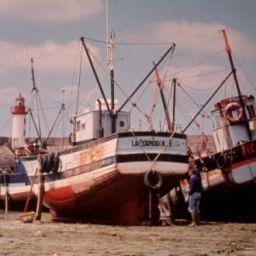
\includegraphics[scale=0.5]{imgs/BoatsColor.jpg}
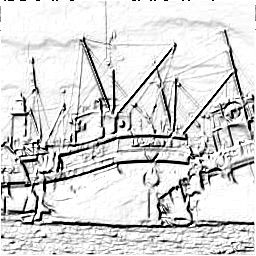
\includegraphics[scale=0.5]{imgs/BoatsColor-sobel-neg.jpg}\\
\texttt{\small Ejemplo del filtro Sobel negado}\\
\vspace{1.0cm}
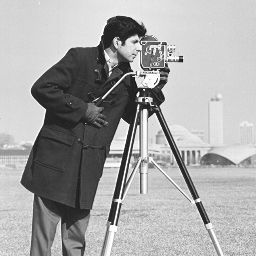
\includegraphics[scale=0.5]{imgs/cameraman.jpg}
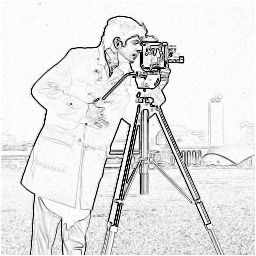
\includegraphics[scale=0.5]{imgs/cameraman-roberts-neg.jpg} \\*
\texttt{\small Ejemplo del filtro Roberts negado}\\
\vspace{1.0cm}
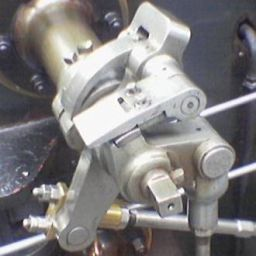
\includegraphics[scale=0.5]{imgs/steam-engine.jpg}
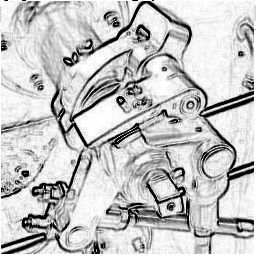
\includegraphics[scale=0.5]{imgs/steam-engine-prewitt-neg.jpg} \\*
\texttt{\small Ejemplo del filtro Prewitt negado} \\
\end{center}
\vspace{1cm}
\pagebreak
\subsection{Medici\'on de performance}
Dado por enunciado, adem\'as de la implementaci\'on de las funciones previamente explicadas, fue necesario realizar 
\keyword{tests de performance} sobre nuestro trabajo, para estos resultados ser comparados con los m\'etodos dados por 
la librer\'ia \keyword{OpenCv} (funci\'on \code{cvSobel}). Tambi\'en nos pareci\'o importante saber qu\'e tan grande era la 
diferencia de \keyword{performance} entre las implementaciones en \keyword{assembler} y C. Al tener todas las 
funciones ya implementadas en ambos lenguajes, vimos interesante la idea de compararlas entre s\'i. La siguiente tabla
muestra la cantidad de ciclos m\'inima y promedio de cada implementaci\'on de los filtros, obtenidos de una muestra de
1000 ejecuciones de cada uno sobre la imagen de prueba \code{lena.bmp}:
\begin{center}
\begin{tabular}{|l|r|r|}
\hline
\multirow{2}{*}{Implementaci\'on}&\multicolumn{2}{|c|}{Ciclos de reloj} \\
\cline{2-3}
&M\'inimo	&	Promedio \\
\hline
\multicolumn{3}{|c|}{Sobel}\\
\hline
Assembler	&	58.720.540	&	60.010.675 \\
\hline
C			&	393.586.848	&	416.838.429 \\
\hline
OpenCv		&	9.338.589	& 	9.797.886 \\
\hline
\multicolumn{3}{|c|}{Roberts}\\
\hline
Assembler	&	34.714.238	&	42.746.947 \\
\hline
C			&	320.676.453	&	336.808.912 \\
\hline
\multicolumn{3}{|c|}{Prewitt}\\
\hline
Assembler	&	60.428.397	&	63.629.648 \\
\hline
C			&	634.337.521	&	664.132.063 \\
\hline
\end{tabular}
\end{center}

Dado a que los algoritmos no fueron pensados para optimizar al m\'aximo en velocidad, se puede ver que \code{cvSobel} 
realiza aproximadamente 6 veces menos de ciclos, obteniendo un mayor rendimiento que la versi\'on en 
\keyword{assembler}. Por otra parte, al comparar los resultados entre las implementaciones de \keyword{assembler} 
y C, las diferencias son estremecedoras: la \keyword{performance} de la versi\'on en \keyword{assembler} es 
aproximadamente 8 veces mejor que la versi\'on en C.

\pagebreak

%\section{Conclusiones}

Con el presente trabajo se muestra que existen formas efectivas, eficientes y simples para el problema de aplicaci\'on 
de filtros espec\'ificos en el marco del procesamiento de im\'agenes. Dichas t\'ecnicas se resumen en un algoritmo simple, 
mas all\'a de que la teor\'ia detr\'as sea m\'as compleja. \\

En cuanto a lo implementado en el trabajo, se infiere directamente una mejora de rendimiento reemplazando el c\'odigo 
escrito en C, por el nuestro escrito en lenguaje ensamblador. M\'as all\'a de cuestiones  y decisiones tomadas que 
afectaron la velocidad final del algoritmo, la diferencia de tiempos entre el lenguaje de alto nivel y el de bajo 
nivel es notable. \\

A\'un as\'i la existencia de un algoritmo m\'as r\'apido y eficaz es evidente como demostr\'o la comparaci\'on de tiempos de 
nuestra implementaci\'on con la funci\'on propia de la librer\'ia. Dicho algoritmo posiblemente est\'e implementado de tal 
manera que aprovecha de mejor forma los registros del procesador, ahorra ciclos con otras instrucciones, o quiz\'a, 
procesando datos en paralelo mediante \code{MMX} o \code{SSE}. Pero implementar un algoritmo de ese estilo resultar\'ia en un c\'odigo m\'as 
complicado y dif\'icil de seguir, perdiendo el sentido original del trabajo. \\

Para finalizar cabe destacar que lo escrito fue dise\~nado para cambiar o agregar f\'acilmente el tipo de operador a 
utilizar en el futuro, respetando a su vez el prototipo de funci\'on dado en el enunciado y que se logr\'o crear una 
herramienta de realce de bordes en im\'agenes que sea general, veloz y efectiva  que al mismo tiempo puede llegar a 
ser \'util en la pr\'actica.
\pagebreak

\section{Manual de usuario}

\subsection{Ayuda r\'apida}

\noindent\textbf{Uso:} \\
\texttt{./bordes [opciones] [archivo] }\\

\noindent\textbf{Opciones:} \\
\texttt{
\begin{tabular}{ll}
-r\#	&	Aplica el operador \#\\
-g	&	Modo gr\'afico \\
--nosse	&	Deshabilita las optimizaciones de SSE \\
--time \# &	Realiza \# repeticiones del operador y muestra información de performance \\
\end{tabular}
}\\

\noindent \textbf{Operadores posibles:}\\
\indent 1: Operador de Roberts \\
\indent 2: Operador de Prewitt \\
\indent 3: Operador de Sobel derivando por X \\
\indent 4: Operador de Sobel derivando por Y \\
\indent 5: Operador de Sobel derivando por X e Y \\
\indent 6: Operador de Frei-Chen

\noindent Si no se especifica un archivo de entrada, se usar\'a \code{lena.bmp} 

\subsection{Descripci\'on}

El programa se puede invocar en modo gr\'afico (\code{-g}) o directo (\code{-r\#}) y opcionalmente una imagen. En modo directo, 
se leer\'a una imagen pasada como par\'ametro o la imagen por defecto (\code{lena.bmp}), se le aplicar\'a el filtro seleccionado 
y se guardar\'a con el nombre original mas un postfijo que indica que filtro fue aplicado y con la extensi\'on original. En modo gr\'afico, 
se puede abrir una imagen y aplicar los filtros, con las teclas del \code{1} al \code{6}, restaurar la imagen en escala de grises 
con la tecla \code{0}, guardar el resultado actual con la tecla \code{s} y deshabilitar las optimizaciones con la tecla \code{o}. 
Se puede salir de este modo con la tecla \code{ESCAPE}. \\

\noindent Tipos de im\'agenes soportados:
\texttt{
\begin{itemize}
\item Windows bitmaps - BMP, DIB 
\item JPEG files - JPEG, JPG, JPE 
\item Portable Network Graphics - PNG 
\item Portable image format - PBM, PGM, PPM 
\item Sun rasters - SR, RAS 
\item TIFF files - TIFF, TIF
\end{itemize}
}
\noindent (extra\'ido de la documentaci\'on de la librer\'ia \keyword{OpenCv})

\subsection{Instrucciones de compilaci\'on}
Dirigirse a la carpeta del c\'odigo (\code{src/}) y ejecutar el comando \code{make}.\pagebreak

%\section{Archivos entregados}
\texttt{
\begin{itemize}
\item informe-xor.pdf
\item src/
	\begin{itemize}
		\item main.c
		\item filters.c
		\item filters.h
		\item asmSobel.asm
		\item asmRoberts.asm
		\item asmPrewitt.asm
		\item apply\_mask.asm
		\item Makefile
	\end{itemize}
\item c-version/
	\begin{itemize}
		\item main.c
		\item filters.c
		\item filters.h
		\item Makefile
	\end{itemize}
\item imgs/
	\begin{itemize}
		\item baboon.jpg
		\item boats.jpg
		\item cameraman.jpg
		\item cln1.jpg
		\item goldhill.jpg
		\item steam-engine.jpg
		\item error/
		\begin{itemize}
			\item error1.png
			\item error2.jpg
		\end{itemize}
	\end{itemize}
\end{itemize}
}


\end{document}
